\documentclass[11pt,a4paper]{article}

% -- Encodage et langue --
\usepackage[utf8]{inputenc}
\usepackage[T1]{fontenc}
\usepackage[french]{babel}

% -- Mise en page --
\usepackage[margin=2.5cm]{geometry}
\usepackage{setspace}
\onehalfspacing

% -- Packages scientifiques --
\usepackage{amsmath,amssymb}
\usepackage{graphicx}
\usepackage{booktabs}
\usepackage{longtable}
\usepackage{multirow}
\usepackage{xcolor}
\usepackage{placeins}
\usepackage{lineno}
\usepackage[labelfont=bf,labelsep=space,figurename=Fig.,tablename=Tableau,justification=justified]{caption}
\usepackage{hyperref}
\hypersetup{
    colorlinks=true,
    linkcolor=blue!60!black,
    citecolor=green!50!black,
    urlcolor=blue!70!black
}

% -- Bibliographie --
\usepackage[authoryear,round]{natbib}

% -- Commandes personnalisees --
\newcommand{\mtb}{\textit{Mycobacterium tuberculosis}}
\newcommand{\ang}{\text{\AA}}
\providecommand{\bibcommenthead}{}

\title{Un site métallique cystéine--histidine--glutamate strictement conservé définit la famille bactérienne DUF501~: inférence évolutive de fonction pour une famille protéique sans parent structural}

\author{Christophe Guyeux$^{1,*}$\\[6pt]
  \parbox{\textwidth}{\centering\small
    $^{1}$Universit\'e Marie et Louis Pasteur, CNRS, institut FEMTO-ST,\\
    F-90000 Belfort, France\\[3pt]
    $^{*}$Auteur correspondant~: \texttt{christophe.guyeux@univ-fcomte.fr}
  }
}

\date{}

% ===========================================================
\begin{document}
\shorthandoff{:;!?}
\linenumbers
\maketitle

\begin{abstract}
\noindent
Des familles protéiques entières n'ont toujours pas de fonction connue, et là où il n'existe ni parent structural ni parent de profil, il ne reste rien d'où transférer une annotation, sinon la trace que la sélection a inscrite dans la famille elle-même. Nous demandons jusqu'où cette trace peut être lue, dans la famille bactérienne DUF501 (un domaine de fonction inconnue~; Pfam PF04417), 4~370 protéines sans terme d'ontologie génique, sans structure résolue et sans parent de repli, pourtant essentielle dans trois genres d'Actinobactéries. Chez son membre tractable Rv1025 de \mtb{}, Cys113, His115 et Glu59 sont occupés dans les 1~472 séquences bactériennes quasi complètes de l'alignement Pfam, sans aucune substitution non conservative parmi les 2~228 examinées~: le site est un trait de toute la famille bactérienne. Sur la structure prédite, les trois chaînes latérales convergent vers un point unique à distance de coordination~; les prédictions holo d'AlphaFold3 y placent un métal divalent, un prédicteur fondé sur la seule géométrie du squelette retrouve le même site, et muter les résidus l'en déplace. Trois signaux supplémentaires l'encadrent~: le bloc de gènes portant DUF501 reste synténique à l'échelle du phylum, dans le cinquième supérieur des blocs de gènes aléatoires, une seconde cavité est conservée indépendamment de lui, et la coévolution ne retrouve que le repli, étant aveugle aux positions invariantes. Trois membres eucaryotes ont perdu le site, et dans les trois la perte est polarisée, la paire cystéine--histidine disparaissant et le glutamate demeurant. Nous proposons que DUF501 est une protéine liant un métal et une métalloenzyme candidate, première hypothèse fonctionnelle pour cette famille~; de nature computationnelle, ce résultat soutient l'occupation métallique plutôt qu'il ne la prouve. La même poche, conservée et essentielle, est une cible antituberculeuse candidate.
\end{abstract}

\textbf{Mots-clés~:} évolution moléculaire, conservation de séquence, génomique comparative, domaine de fonction inconnue, métalloprotéine, \textit{Mycobacterium tuberculosis}

\section{Introduction}

Des familles protéiques entières n'ont toujours pas de fonction connue. Des milliers de familles Pfam ne sont définies que par un domaine de fonction inconnue (DUF), et elles ne constituent pas un catalogue de curiosités marginales~: les gènes réduits à un DUF sont essentiels chez les bactéries à des taux comparables à ceux des gènes annotés \citep{goodacre2014dufessential}, et ces familles sont identifiées de longue date comme une lacune persistante de l'annotation des génomes séquencés \citep{bateman2010dufs}. L'obscurité structurale est tout aussi tenace, couvrant des régions et des protéines entières pour lesquelles on ne dispose ni de structure expérimentale ni de modèle confiant \citep{perdigao2015darkproteome}.

La fonction s'assigne ordinairement par transfert, depuis un homologue d'activité connue, un parent structural ou un motif catalytique reconnu. Quand une famille n'offre aucun des trois, le transfert n'a plus de prise, et la seule information qui subsiste sur ce que font ses membres est la trace que la sélection a inscrite dans la famille elle-même~: des positions qui ne changent jamais, des paires de positions qui changent ensemble, des arrangements de gènes qui survivent aux réarrangements génomiques. Chacune porte un type de preuve différent et diversement limité, et la question pratique est de savoir jusqu'où les pousser avant qu'elles ne cessent de distinguer une contrainte fonctionnelle de la contrainte ordinaire qui maintient une protéine repliée.

DUF501 (Pfam PF04417, InterPro IPR007511, groupe orthologue COG1507, orthologie KEGG K09009) est une famille exactement de ce type~: 4~370 protéines réparties sur 5~484 taxons, sans terme d'ontologie génique, sans structure résolue expérimentalement et sans annotation enzymatique. Elle est en même temps non superflue, ce qui est inhabituel pour une famille sombre, le gène DUF501 étant rapporté essentiel chez \mtb{} (Rv1025) \citep{dejesus2017essentiality}, \textit{Corynebacterium glutamicum} (cgp\_1113) et \textit{C.\ diphtheriae} (DIP0919) \citep{goodall2023diphtheriae}~; ce qu'il fait n'est donc redondant avec rien d'autre dans ces génomes.

Son membre chez \mtb{}, Rv1025, protéine de 155 résidus, est un point d'entrée favorable pour une analyse évolutive de la famille. Il est échantillonné bien plus profondément que la plupart des protéines bactériennes, avec cinq sites polymorphes sur 145~209 génomes cliniques et une unique substitution synonyme le séparant du groupe externe \textit{M.\ canettii}, de sorte que l'extrémité récente de son histoire évolutive est dense. Il est modélisé avec une grande confiance (confiance moyenne par résidu d'AlphaFold, pLDDT, 95,3), de sorte que la conservation à l'échelle de la famille peut se lire sur une structure et non sur la seule séquence. Et il se situe dans un bloc de quatre gènes, \textit{eno} (Rv1023, énolase)--\textit{divIC} (Rv1024, protéine de division cellulaire de la famille FtsB/DivIC)--\textit{Rv1025}--\textit{ppx2} (Rv1026, une exopolyphosphatase \citep{chuang2015rv1026ppx2,choi2012ppxgppa,tiwari2019polyp}), dont les membres relèvent de voies sans rapport (glycolyse, division, métabolisme des polyphosphates), si bien que le contexte génomique n'assigne rien à lui seul. Que la protéine soit en outre fortement vulnérable à l'inactivation transcriptionnelle \citep{bosch2021vulnerability} et détectée par spectrométrie de masse en fait un objet réel et expérimentalement accessible, et non un cadre de lecture prédit.

Nous lisons ici la trace évolutive de DUF501 à quatre échelles et demandons ce que chacune soutient. Nous établissons d'abord que la famille n'a ni parent structural ni parent de profil de séquence, de sorte que le transfert par homologie est réellement indisponible. Nous montrons ensuite que le bloc de gènes portant DUF501 reste synténique à travers les Actinobactéries dans la partie haute de la distribution des blocs de quatre gènes tirés au hasard, alors que la protéine ne forme aucun complexe binaire stable avec son voisin de division invariant, si bien que l'arrangement conservé n'est pas la signature d'une paire physique~; que le repli porte une constellation quasi invariante Cys--His--Glu dont la géométrie apo et la modélisation holo indiquent l'une et l'autre un site à métal divalent~; et que ce site est présent dans toute la famille, puisqu'il est occupé dans chaque séquence bactérienne quasi complète de la famille, ce qui autorise à énoncer pour la famille entière une hypothèse dérivée d'un membre unique. Nous examinons ensuite ce qu'ajoute la coévolution des résidus, et pourquoi elle ajoute peu à un site dont la propriété définissante est de ne pas varier, puis nous rapportons la perte partielle et polarisée de ce même site chez trois membres de la branche eucaryote de la famille. Nous terminons sur ce qui en découle pour \mtb{}, chez qui cette poche conservée et essentielle est une cible antituberculeuse candidate.

\section{Matériel et méthodes}

\paragraph{Séquence, annotation et conservation.} La séquence protéique de Rv1025 (UniProt P96375, 155 aa) et ses voisins d'opéron ont été extraits de la référence H37Rv (NC\_000962.3) \citep{cole1998genome}. Les statistiques au niveau de la famille (nombre de membres et de taxons, termes d'ontologie génique, structures PDB associées) ont été récupérées depuis InterPro/Pfam \citep{paysanlafosse2023interpro} et l'orthologie depuis eggNOG \citep{huertacepas2019eggnog}. L'essentialité et la vulnérabilité proviennent des cribles publiés par transposon \citep{dejesus2017essentiality} et CRISPRi \citep{bosch2021vulnerability}~; l'essentialité inter-genres a été obtenue depuis l'étude du génome essentiel de \textit{Corynebacterium diphtheriae} \citep{goodall2023diphtheriae}. La conservation résidu par résidu a été calculée à partir de l'alignement multiple profond généré par AlphaFold3 pour Rv1025 (8~700 séquences)~; après retrait des états d'insertion, chaque position de la requête a été notée par la fraction de séquences sans gap correspondant au résidu de la requête.

\paragraph{Modèle de structure et recherche structurale.} Le modèle AlphaFold de Rv1025 (AlphaFold DB v6, AF-P96375-F1, pLDDT moyen 95,3) \citep{jumper2021alphafold,varadi2022afdb} a été recherché avec Foldseek \citep{vankempen2024foldseek} contre les bases complètes PDB100, AlphaFold/Swiss-Prot et CATH50 (mode 3Di+AA). Une recherche complémentaire profil--profil (HMM--HMM) a été menée avec HHpred \citep{zimmermann2018hhpred} contre PDB\_mmCIF70, Pfam-A et SCOPe70.

\paragraph{Synténie à travers les Actinobactéries.} Les quatre protéines de l'opéron ont été interrogées par \texttt{tblastn} \citep{camacho2009blast} (e-value $\leq 10^{-5}$) contre 63 génomes de référence~: 48 espèces de \textit{Mycobacterium} non tuberculeuses, \textit{M.\ canettii} et \textit{M.\ bovis} comme témoins, dix Actinobactéries non-\textit{Mycobacterium} couvrant les Corynebacteriales, Streptomycetales, Bifidobacteriales, Propionibacteriales et Micrococcales, et \textit{Escherichia coli} et \textit{Bacillus subtilis} comme négatifs hors phylum. Pour chaque génome, le meilleur hit par requête a été retenu~; la synténie a été évaluée par co-localisation et ordre des gènes autour de l'ancre DUF501. Pour tester si la synténie de l'opéron dépasse le niveau de fond du génome, nous avons tiré 90 blocs aléatoires de quatre gènes co-directionnels de H37Rv et noté chacun, par la même procédure \texttt{tblastn}, à travers les onze Actinobactéries distantes (non-\textit{Mycobacterium}). Pour séparer la conservation de l'arrangement de la conservation des gènes, la notation a été conditionnée sur l'orthologie~: pour chaque bloc, nous avons compté les génomes où les quatre orthologues étaient trouvés (présents) et, parmi ceux-ci, les génomes où ils étaient synténiques (contig unique, étendue $\leq 8$~kb, ordre cohérent)~; la statistique par bloc est la fraction synténique sachant présent, et l'opéron a été placé dans la distribution nulle résultante ($p$ empirique à partir de la fraction de blocs aléatoires au moins aussi synténiques). Un schéma du bloc le long de la taxonomie des Actinobactéries a été tracé avec Matplotlib (Ressource en ligne~13).

\paragraph{Modélisation de complexes et holo.} AlphaFold3 \citep{abramson2024alphafold3} a été exécuté via l'AlphaFold Server avec une graine de modèle fixe, retournant cinq modèles par tâche. Les interactions putatives ont été testées comme hétérodimères (Rv1025 avec DivIC~; témoins de spécificité Rv1025 avec Énolase et avec Ppx2~; témoin positif DivIC avec la protéine du divisome FtsQ, Rv2151c) et évaluées par le pTM d'interface (ipTM) et l'erreur d'alignement prédite minimale inter-chaînes, sur les cinq modèles par tâche. Le site métallique a été testé par des prédictions holo de Rv1025 avec un seul ion Zn, Fe ou Mn~; la coordination a été mesurée sur le modèle le mieux classé comme les distances entre l'ion et les atomes donneurs candidats, avec le pLDDT par ion comme estimation de confiance. Comme témoin négatif, les trois ligands ont été mutés en alanine (C113A/H115A/E59A) et la prédiction holo répétée. Comme contrôle de robustesse du résultat DivIC, cinq composants supplémentaires du divisome (FtsZ, FtsW, PbpB/FtsI, FtsK, SepF) ont été criblés comme hétérodimères avec Rv1025 en utilisant Boltz-2 \citep{passaro2025boltz2} exécuté localement sur CPU, en réutilisant l'alignement multiple de Rv1025 généré par AlphaFold3 et la paire DivIC--FtsQ comme témoin positif interne au panel~; parce que l'inférence Boltz-2 mono-modèle sur CPU est un prédicteur distinct, plus bruité, que l'AlphaFold Server, ces résultats sont rapportés séparément et ne sont pas mêlés aux chiffres AlphaFold3. Un homodimère direct de Rv1025, avec et sans les deux ions Fe holo, a de même été testé par AlphaFold3 pour demander si une seconde sous-unité pourrait compléter la sphère de coordination du métal en trans. L'analyse des structures a utilisé Biopython \citep{cock2009biopython}~; les figures moléculaires ont été rendues avec PyMOL.

\paragraph{Conservation de la triade à l'échelle de la famille.} L'alignement Pfam complet de PF04417 (version PF04417.18~; 2~228 segments alignés issus de 2~204 protéines distinctes, 471 colonnes) a été récupéré depuis l'API InterPro et utilisé tel quel, sans réalignement~; il a été construit sur la base de séquences Pfam (environ 91 millions de séquences) et couvre donc environ la moitié des membres actuels de la famille dans InterPro. Rv1025 étant elle-même un membre (P96375/16--137), les colonnes de l'alignement correspondant à Glu59, Cys113 et His115 ont été localisées en parcourant sa ligne alignée, et chaque séquence a ensuite été lue à ces trois colonnes. Les séquences ont été considérées quasi complètes lorsque leur longueur alignée atteignait 90~\% de la longueur médiane des membres porteurs de la triade, ce qui sépare les substitutions authentiques des gaps de fragments~; une substitution conservative a été définie comme la rétention de la chimie de coordination (Asp pour Glu). Les lignées taxonomiques ont été obtenues depuis l'API REST d'UniProt pour chaque accession, et l'identité à Rv1025 a été calculée sur les colonnes où les deux séquences sont sans gap. 24 accessions figurant dans l'alignement par deux segments distincts, l'état du site a été coté par protéine et non par segment aligné~: une protéine compte comme porteuse du site quand l'union de ses segments porte les trois résidus. Pour chaque accession dont les segments ne portaient pas la triade complète, la séquence UniProt entière a été ajoutée au profil par MAFFT v7.526 \citep{katoh2013mafft} sous \texttt{--add --keeplength}, qui préserve les 471 colonnes de référence et permet donc de relire les mêmes trois colonnes~; dix accessions dont le hit Pfam porte déjà la triade complète ont suivi la procédure identique, en contrôle positif.

\paragraph{Analyse de co-évolution.} La co-évolution résiduelle a été calculée sur le même alignement de 8~700 séquences par analyse de couplage direct en champ moyen \citep{morcos2011dca}~: les séquences ont été repondérées à 80~\% d'identité, les fréquences régularisées par un pseudo-compte de 0,5, et les couplages obtenus par inversion de la matrice de covariance, convertis en normes de Frobenius dans la jauge à somme nulle et corrigés du fond par la correction du produit moyen \citep{dunn2008apc}. Les colonnes à plus de 50~\% de gaps et les paires séparées de moins de cinq résidus ont été exclues. Les paires prédites ont été comparées au modèle apo par les distances C$\beta$--C$\beta$, les contacts étant définis à 8~\ang{}~; les paires au-delà de 15~\ang{} ont été considérées comme non expliquées par le monomère. L'accessibilité au solvant relative a utilisé les aires de Shrake--Rupley normalisées aux maxima de \citet{tien2013maxasa}. L'enrichissement des couplages entre les deux poches a été testé contre un null apparié en distance de 10~000 ré-échantillonnages, la force de couplage décroissant avec la distance.

\paragraph{Prédiction orthogonale du site métallique et druggabilité.} Pour évaluer le site métallique indépendamment du signal de conservation et du placement métallique appris par AlphaFold, le modèle apo a été analysé avec BioMetAll \citep{sanchezaparicio2021biometall}, qui identifie les sites de liaison métallique à partir de la seule préorganisation du squelette, et avec AlphaFill \citep{hekkelman2023alphafill}, qui transplante ligands et ions depuis des structures holo homologues. La détection de poches et la notation de druggabilité du modèle apo ont utilisé fpocket \citep{leguilloux2009fpocket}~; chaque poche détectée a été rattachée au site métallique par la distance minimale entre ses centres de sphères alpha et les atomes donneurs Cys113/His115/Glu59.

\paragraph{Accessibilité du site métallique.} La fonction de notation de fpocket, pondérée par hydrophobicité, n'étant pas conçue pour des sites métalliques polaires, l'accessibilité de l'ion coordonné a plutôt été mesurée géométriquement, indépendamment de cette fonction de notation. Sur chacun des cinq modèles holo par ion (Zn, Fe, Mn~; eau et tout autre atome non protéique exclus dans tous les cas), 4~000 directions ont été lancées depuis l'ion à 2,1~\ang{}~; une direction était notée \emph{ouverte} si aucun atome protéique ne se trouvait à moins de 2,4~\ang{} de la sonde (répété aux seuils 2,6 et 2,8~\ang{} comme contrôle de robustesse) et \emph{tournée vers le solvant} si elle atteignait de plus 10~\ang{} depuis l'ion sans passer à moins de 1,9~\ang{} d'aucun atome. La même procédure a été appliquée, avec les seuils identiques, à quatre structures de calibration~: trois sites de zinc catalytiques validés (anhydrase carbonique II humaine, PDB 1CA2 \citep{eriksson1988carbonicanhydrase}~; thermolysine, PDB 8TLN \citep{holland1992thermolysin}~; la désacétylase bactérienne LpxC, PDB 4MDT \citep{clayton2013lpxc}) et un site de zinc structural, non catalytique (le domaine en doigt de zinc Zif268, PDB 1ZNF \citep{lee1989zincfinger}). Pour séparer l'accessibilité authentique d'un biais possible des modèles AlphaFold vers un empilement plus lâche que les structures cristallines, la même mesure a été répétée sur les modèles AlphaFold DB des deux protéines de calibration à site actif d'origine cristallographique (anhydrase carbonique II, thermolysine), le métal étant transplanté sur le modèle par superposition de Kabsch des atomes C$\alpha$ appariés après résolution de tout décalage de numérotation entre les séquences cristallographiques et UniProt.

Les analyses bioinformatiques, les interrogations de bases de données et le recoupement bibliographique sous-tendant cette étude ont été menés au sein d'un environnement de travail bioinformatique augmenté par IA, Claude Code (Anthropic), faisant fonctionner le modèle de langage Claude Sonnet~5 comme agent d'analyse interactif sous direction humaine continue. Chaque script, test statistique et affirmation numérique produits dans cet environnement a été retracé de façon indépendante jusqu'à sa donnée brute, sa publication primaire ou son enregistrement de base de données sous-jacents avant d'être rapporté ici, suivant la discipline de vérification décrite tout au long de cette section~; l'auteur correspondant a conçu l'étude, spécifié et relu chaque analyse, et assume l'entière responsabilité de l'exactitude de son contenu.

\section{Résultats}

\subsection{Rv1025 et la famille DUF501 sont essentielles mais non caractérisées à travers les Actinobactéries}

Rv1025 est un authentique produit de gène, bien étayé~: elle est essentielle par mutagenèse par transposon \citep{dejesus2017essentiality}, fortement vulnérable à l'inactivation par CRISPRi (indice de vulnérabilité $-5,7$, IC 95~\% $-6,2$ à $-5,2$) \citep{bosch2021vulnerability}, détectée par spectrométrie de masse, quasi invariante à travers les isolats cliniques (seulement cinq sites polymorphes sur 145~209 génomes, aucun disruptif), et prédite très bien repliée (pLDDT moyen 95,3). Cette invariance se maintient à des échelles phylogénétiques plus profondes~: Rv1025 diffère de l'extra-groupe immédiat \textit{M.\ canettii} par une seule substitution synonyme, et c'est un gène du cœur du genre retenu à travers toutes les espèces de \textit{Mycobacterium} échantillonnées. (Ne disposant que de cinq sites intra-complexe et d'une substitution vis-à-vis de l'extra-groupe, nous rapportons ces chiffres comme des comptes de sites ségrégeants/substitués plutôt que comme des ratios $dN/dS$ ou $pN/pS$, sous-puissants à cet échantillonnage et qui sur-interpréteraient un basculement à un seul variant.) Pourtant ni Rv1025 ni sa famille n'ont d'annotation fonctionnelle. La famille Pfam DUF501 (PF04417, InterPro IPR007511) n'est décrite que comme « famille de protéines bactériennes non caractérisées », comprenant 4~370 protéines à travers 5~484 taxons sans terme d'ontologie génique associé et, surtout, sans structure résolue expérimentalement~; l'orthologie eggNOG (COG1507) et l'orthologie KEGG (K09009) sont de même « fonction inconnue ». L'essentialité, cependant, n'est pas idiosyncrasique à \mtb{}~: le gène DUF501 est rapporté essentiel dans trois genres d'Actinobactéries, \mtb{} (Rv1025), \textit{Corynebacterium glutamicum} (cgp\_1113) et \textit{C.\ diphtheriae} (DIP0919) \citep{goodall2023diphtheriae}, identifiant DUF501 comme une fonction cœur conservée, non redondante, dont la nature moléculaire est inconnue.

\subsection{DUF501 n'a aucun homologue structural ou de profil de séquence détectable}

Pour chercher une fonction par la structure, nous avons interrogé le modèle AlphaFold à haute confiance de Rv1025 contre des bases de données structurales complètes avec Foldseek. Aucun homologue significatif n'a été trouvé~: la recherche AlphaFold/Swiss-Prot n'a retourné aucun hit, PDB100 a retourné une seule correspondance partielle et non significative (26~\% de la requête à 24~\% d'identité), et CATH50 a retourné cinq hits marginaux (13--19~\% d'identité, $e \geq 0,01$) dispersés sur cinq replis \emph{différents} sans convergence. Une recherche profil--profil complémentaire avec HHpred, plus sensible à l'homologie distante, n'a de même retourné aucun hit significatif au-delà de la famille elle-même~: les seules correspondances à haute probabilité étaient des auto-hits vers les profils DUF501 (COG1507 et PF04417, probabilité 100~\%), tandis que tout autre hit tombait sous 56~\% de probabilité avec des E-values $\geq 18$ et ne convergeait vers aucun repli caractérisé. DUF501 adopte donc un repli non représenté dans le PDB ni dans CATH et n'a aucun parent de profil de séquence détectable~; le modèle de Rv1025 est, à notre connaissance, le premier représentant structural de la famille. Le transfert par homologie ne peut assigner sa fonction.

\subsection{L'opéron \textit{eno}--\textit{divIC}--\textit{Rv1025}--\textit{ppx2} est conservé à travers le phylum des Actinobactéries}

Bien que l'opéron mélange des voies sans rapport, son arrangement est néanmoins fortement conservé. En interrogeant les quatre protéines contre 63 génomes de référence, le bloc complet de quatre gènes a été retrouvé intact et dans le même ordre, avec \textit{divIC} toujours voisin immédiat de \textit{Rv1025}, dans 61 génomes sur 63 (Figure~\ref{fig:synteny})~: le genre \textit{Mycobacterium} entier (48/48 espèces, y compris les génomes réduits de \textit{M.\ leprae} et \textit{M.\ lepromatosis}, qui retiennent le bloc entier), l'ordre des Corynebacteriales (\textit{Corynebacterium}, \textit{Nocardia}, \textit{Rhodococcus}, \textit{Gordonia}, \textit{Tsukamurella}, \textit{Mycobacteroides}), et des représentants des Streptomycetales, Bifidobacteriales, Propionibacteriales et Micrococcales. DUF501 était entièrement absent des deux négatifs hors phylum (\textit{E.\ coli}, \textit{B.\ subtilis}). De façon cohérente, la famille est fortement enrichie dans ce phylum sans y être confinée~: sur les 4~378 protéines DUF501 répertoriées dans InterPro lorsque cette répartition taxonomique a été relevée (le décompte de l'entrée varie de quelques protéines d'une version à l'autre, d'où 4~370 plus haut), 3~830 (87~\%) sont des Actinomycetota, suivies de Pseudomonadota (264), des entrées eucaryotes dispersées (179) et une poignée de Bacillota (24) \citep{paysanlafosse2023interpro}. La conservation d'un bloc de gènes ordonné sur des centaines de millions d'années, dans des génomes dont l'ordre des gènes est par ailleurs largement réarrangé, pointe vers une association fonctionnelle entre ces gènes plutôt qu'une co-hérédité passive. Pour vérifier que ceci ne relève pas simplement du niveau de fond de la conservation de l'ordre des gènes à l'échelle du génome, nous avons appliqué le même test de synténie à 90 blocs aléatoires de quatre gènes de H37Rv à travers les onze Actinobactéries distantes non-\textit{Mycobacterium}, en conditionnant sur l'orthologie de sorte que seul l'arrangement, pas la conservation des gènes, soit noté (Méthodes). Parmi les 43 blocs dont les gènes sont largement conservés, la synténie sachant l'orthologie est préservée à une médiane de 0,55 (moyenne 0,47), contre 1,00 pour l'opéron~: le bloc \textit{eno}--\textit{divIC}--\textit{Rv1025}--\textit{ppx2} est entièrement synténique partout où ses gènes sont présents et se situe dans le cinquième supérieur des blocs conservés (8 des 43 aussi synténiques ou plus~; Ressource en ligne~4). Son arrangement est donc maintenu bien au-dessus du niveau de fond de co-hérédité passive, bien que, comme attendu pour les Actinobactéries riches en opérons, il ne s'agisse pas d'un outlier unique. Le bloc est retenu de \mtb{} à \textit{Bifidobacterium} (identité de Rv1025 de 100~\% à 51~\%) le long de la taxonomie des Actinobactéries (Ressource en ligne~13).

\begin{figure}[htbp]
\centering
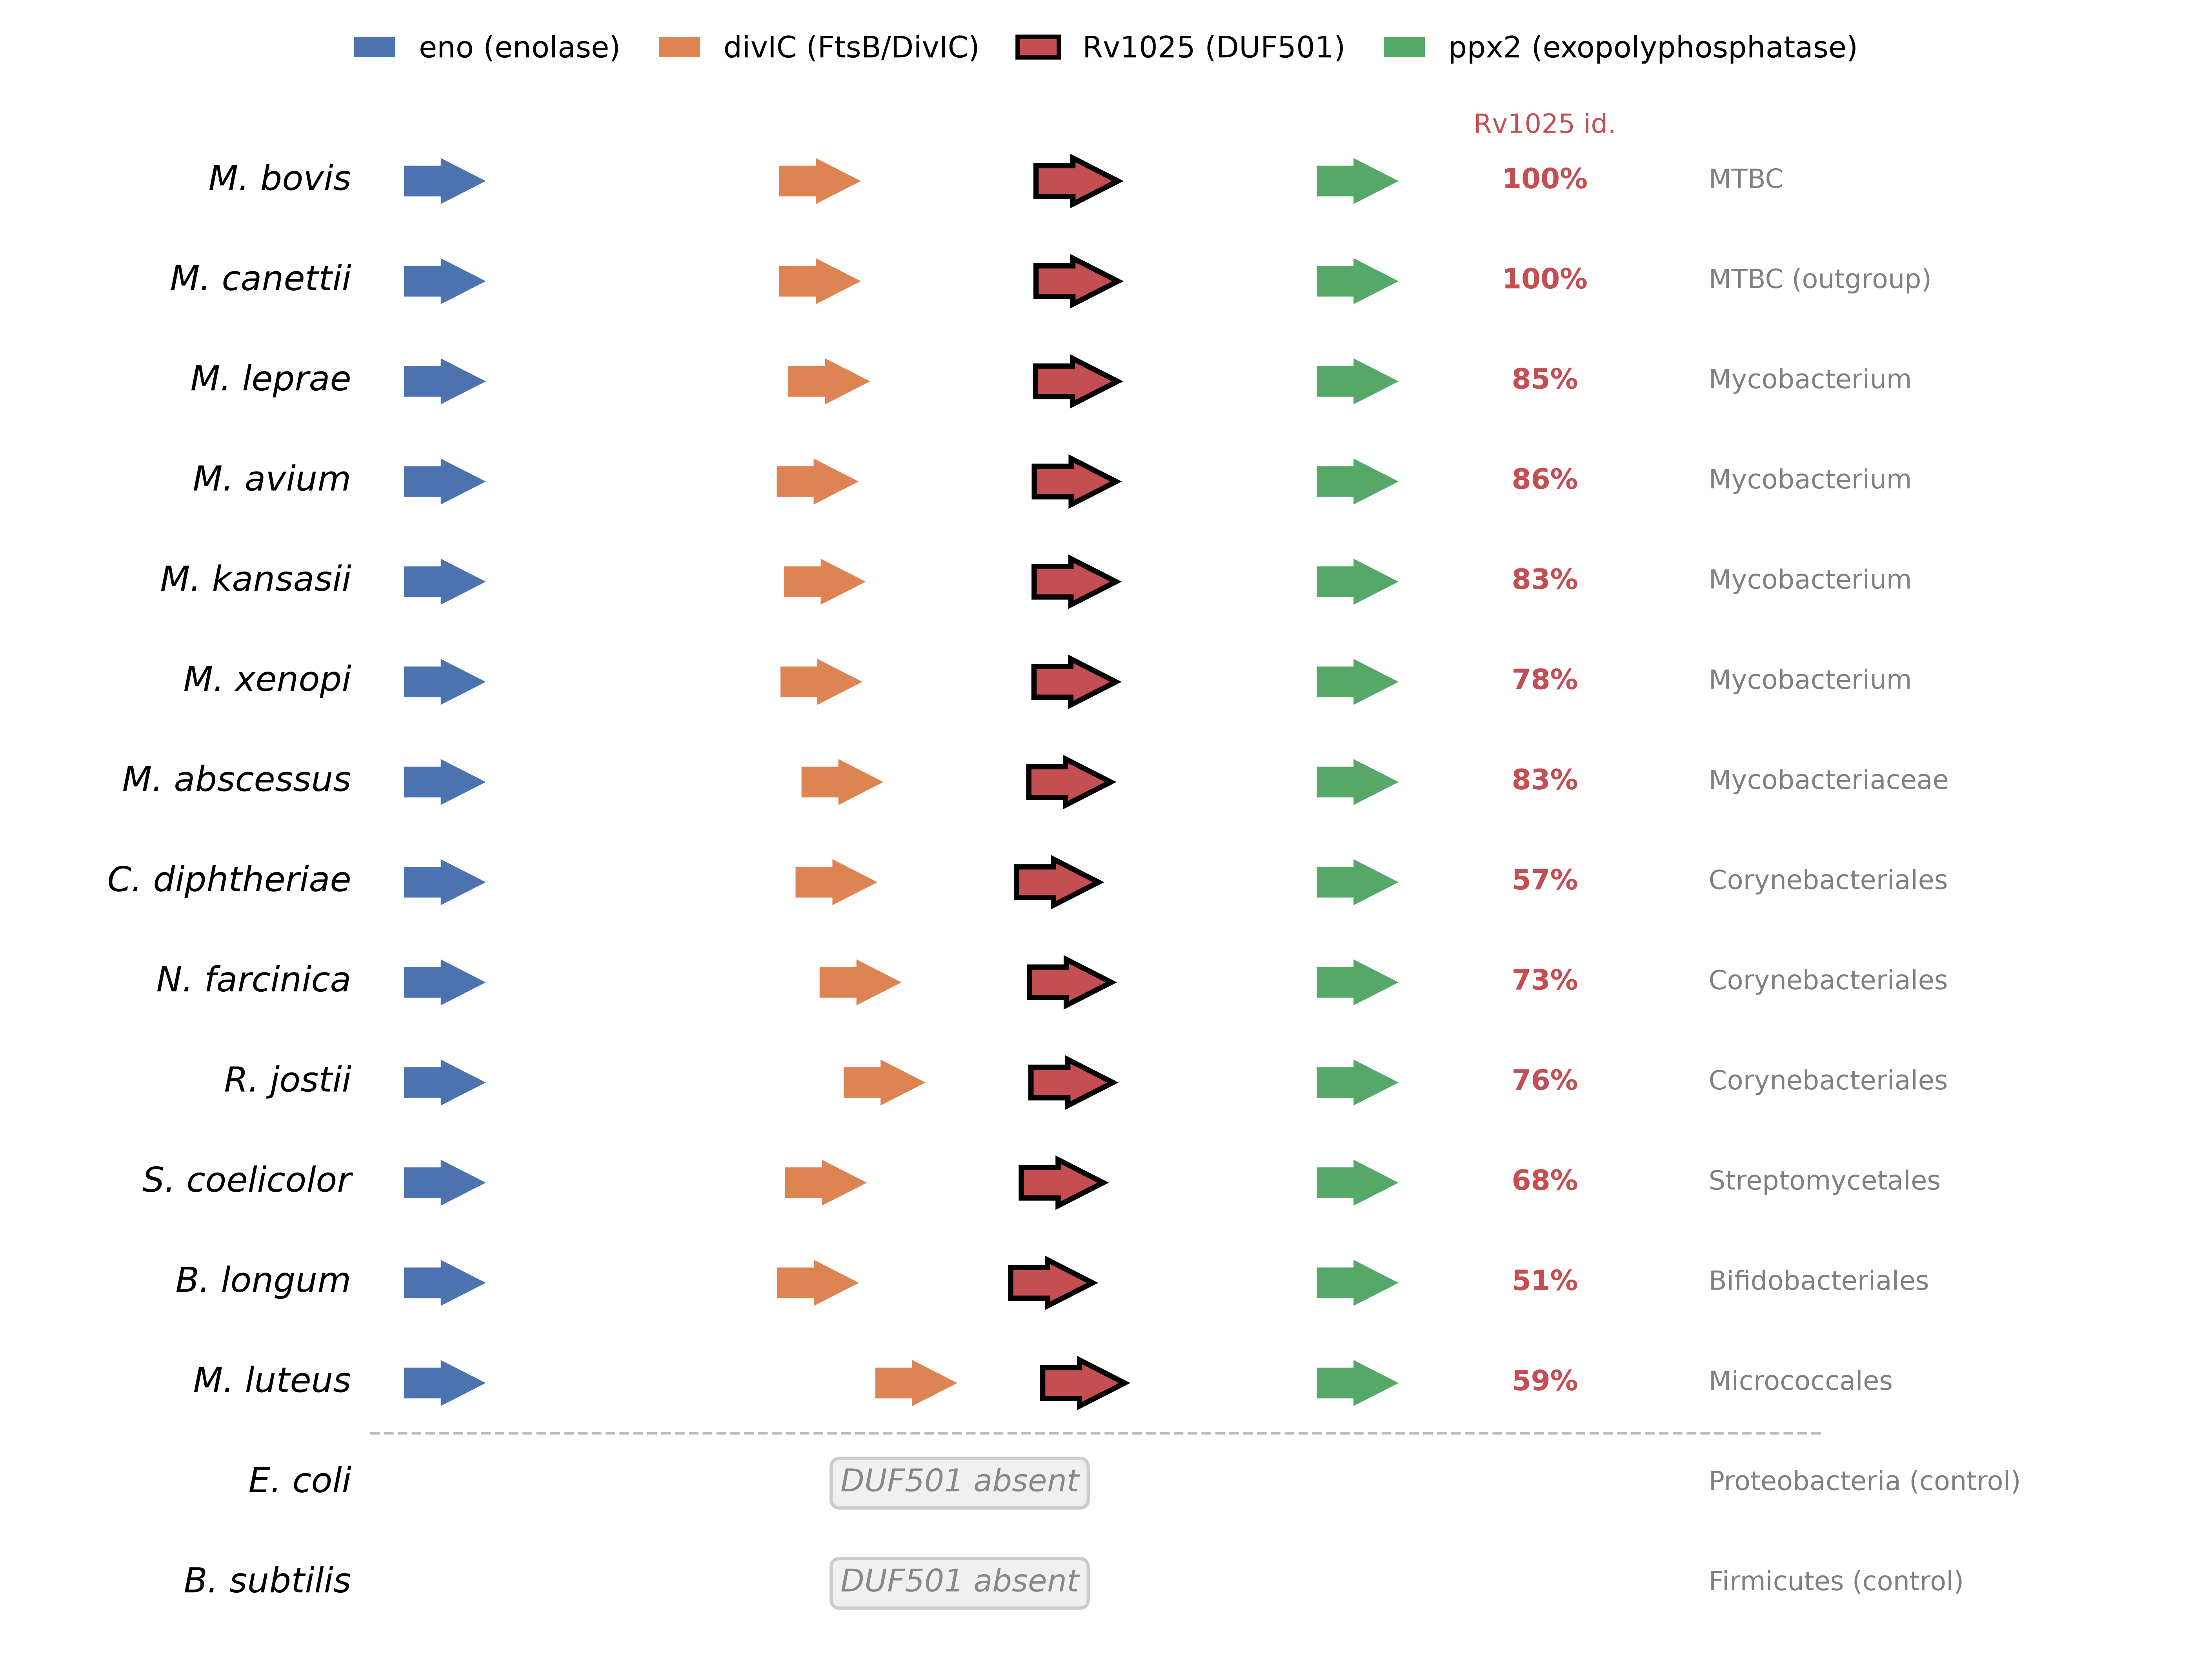
\includegraphics[width=\textwidth]{figures/figure2_synteny.png}
\caption{L'opéron \textit{eno}--\textit{divIC}--\textit{Rv1025}--\textit{ppx2} est une unité génomique conservée à travers les Actinobactéries. Les génomes représentatifs sont ordonnés du complexe \textit{M.\ tuberculosis} (en haut) aux ordres d'Actinobactéries distants, avec deux négatifs hors phylum en bas. L'ordre des gènes est normalisé pour que l'opéron se lise de gauche à droite (dans plusieurs génomes, p.~ex.\ \textit{N.\ farcinica}, \textit{S.\ coelicolor}, le bloc se trouve sur le brin opposé). \textit{divIC} (famille FtsB/DivIC) est le voisin immédiat invariant de \textit{Rv1025} (DUF501, encadré). L'identité en acides aminés de Rv1025 à \mtb{} est indiquée à droite~; DUF501 est absent de \textit{E.\ coli} et de \textit{B.\ subtilis}. Les données complètes pour les 63 génomes figurent dans la Ressource en ligne~1}
\label{fig:synteny}
\end{figure}

\subsection{Rv1025 ne forme pas de complexe binaire stable avec DivIC}

DivIC (famille FtsB/DivIC) étant le voisin synténique invariant, nous avons testé une interaction physique directe avec AlphaFold-Multimer. La prédiction fut négative et spécifique. Comme témoin positif, la paire établie du divisome DivIC--FtsQ a été retrouvée de façon reproductible (ipTM 0,38 sur les cinq modèles, erreur d'alignement prédite minimale inter-chaînes de 5,1~\ang{}), montrant que le test peut détecter une interface de division authentique, quoiqu'avec un plafond d'ipTM modeste, typique des interfaces de petites protéines membranaires. Face à cette calibration, Rv1025--DivIC a échoué~: son meilleur ipTM était de 0,25 mais s'effondrait à 0,08 entre modèles (pas de pose convergente), avec une erreur inter-chaînes de 14,7~\ang{}, au niveau des témoins de spécificité Rv1025--Énolase (0,19) et Rv1025--Ppx2 (0,17). La conservation synténique profonde reflète donc une association fonctionnelle ou une co-régulation, non un hétérodimère stable démontrable avec DivIC (Figure~\ref{fig:afmm}).

\begin{figure}[htbp]
\centering
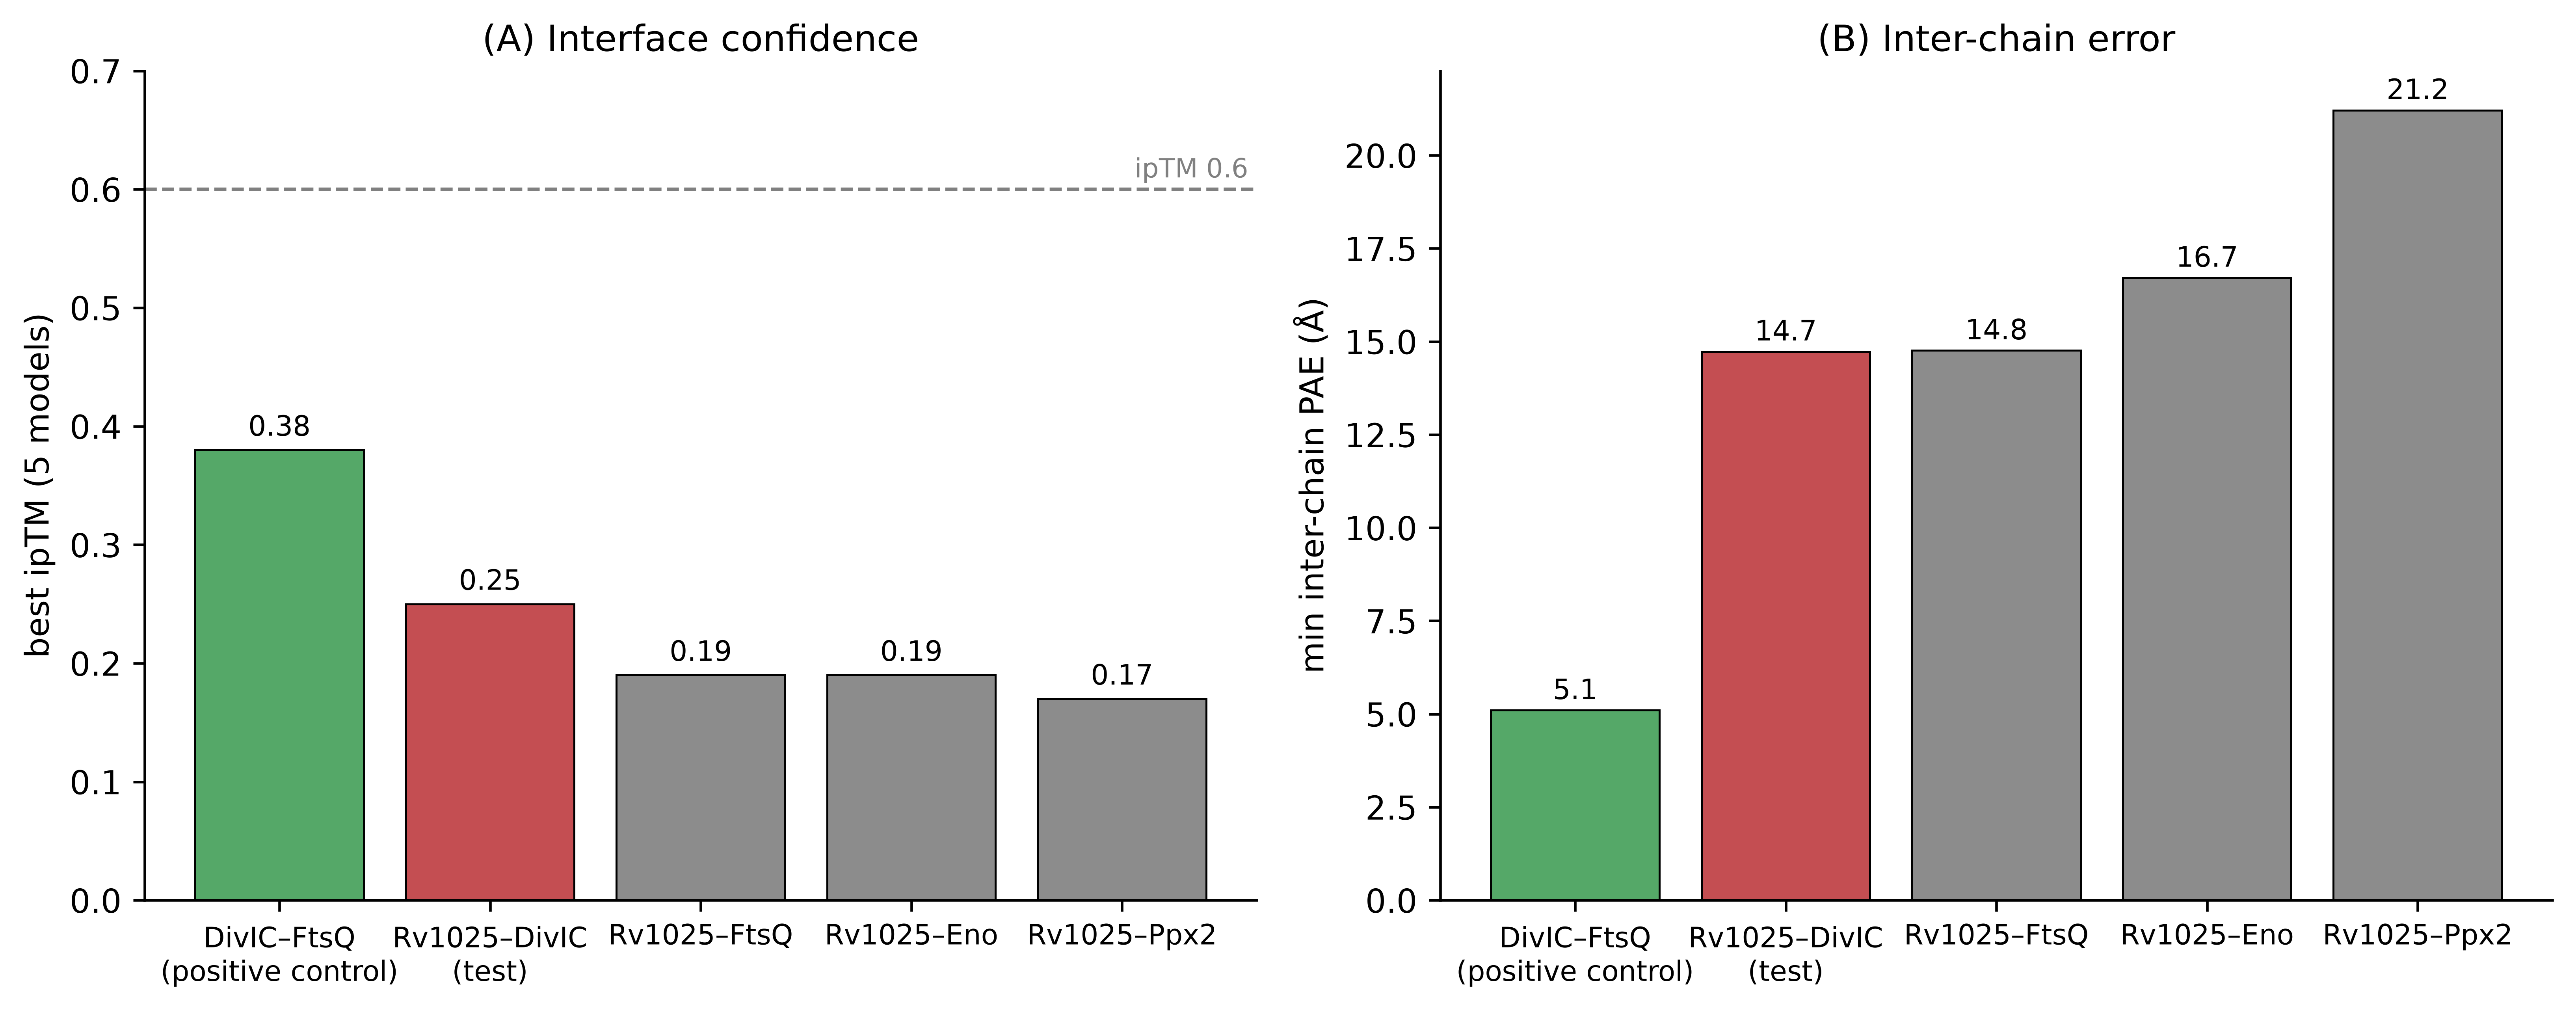
\includegraphics[width=0.92\textwidth]{figures/figure3_afmultimer.png}
\caption{AlphaFold-Multimer ne soutient pas de complexe direct Rv1025--DivIC. \textbf{(A)} Meilleur pTM d'interface (ipTM) sur les cinq modèles et \textbf{(B)} erreur d'alignement prédite (PAE) minimale inter-chaînes pour chaque paire. La paire établie du divisome DivIC--FtsQ (témoin positif, vert) est la seule à combiner un ipTM plus élevé avec un PAE inter-chaînes faible (5,1~\ang{}), indiquant une interface authentique~; le test Rv1025--DivIC (rouge) et les témoins de spécificité (Rv1025 avec FtsQ, Énolase, Ppx2~; gris) montrent tous un ipTM faible et un PAE inter-chaînes élevé}
\label{fig:afmm}
\end{figure}

\subsection{Une triade quasi invariante Cys--His--Glu forme un site métallique soutenu par le modèle holo AlphaFold3}

Nous nous sommes ensuite tournés vers la conservation. Sur un alignement de 8~700 séquences homologues, 23 résidus sont quasi invariants ($\geq 90~\%$ d'identité à la requête)~; parmi eux, plusieurs de type catalytique, notamment Cys113 et His115 (tous deux conservés à 100~\%) et Glu59 (99~\%). L'invariance des trois résidus se maintient aussi sur l'alignement seed Pfam curé (39 séquences), indépendamment de la redondance du grand alignement, où Cys113, His115 et Glu59 sont chacun pleinement conservés (Ressource en ligne~11). Sur le modèle AlphaFold, ces trois résidus forment un groupement compact au sein d'une crevasse. En mesurant leur géométrie, les atomes donneurs des chaînes latérales (Cys-S$\gamma$, His-N$\delta$1, Glu-O$\varepsilon$) convergent vers un point commun à $\sim$2,3~\ang{} de chacun, la signature d'un site de coordination métallique mononucléaire plutôt que d'un relais de triade catalytique linéaire.

Pour tester cela, nous avons exécuté des prédictions holo AlphaFold3 de Rv1025 avec un seul ion Zn, Fe ou Mn. Dans tous les cas, l'ion a été placé dans le site Cys113--His115--Glu59 à des distances métal--ligand canoniques et avec une confiance par ion très élevée (Table~\ref{tab:metal}~; Figure~\ref{fig:site})~: 2,25--2,47~\ang{} aux trois donneurs, pLDDT par ion 94--98, de façon reproductible, le fer donnant le modèle le plus confiant. La coordination protéique est incomplète~: seuls trois ligands protéiques (avec une possible contribution bidentate de Glu59) engagent le métal, laissant des positions de coordination ouvertes faisant face à la poche bordée par les résidus conservés et chargés de seconde sphère Lys112 et Arg92. Un tel métal incomplètement coordonné par la protéine et ouvert au solvant est plus cohérent avec un centre métallique catalytique qu'avec un centre purement structural. Comme témoin de spécificité, nous avons muté les trois ligands en alanine (C113A/H115A/E59A) et répété la prédiction holo. Le repli était préservé (pLDDT moyen 96), mais le métal n'occupait plus le site~: il s'est déplacé de 16--22~\ang{} vers un groupement de surface non conservé (Cys20/His48/Glu24, à 74/20/8~\% de conservation dans la famille contre 99--100~\% pour la vraie triade). Abolir la triade conservée abolit donc la liaison métallique à ce site, indiquant que le placement de type sauvage est spécifique à Cys113--His115--Glu59 plutôt qu'un artefact de surface arbitraire. Le déplacement montre aussi qu'AlphaFold3 accommodera un métal divalent à tout groupement Cys/His/Glu approprié, si bien que la confiance par ion seule n'est pas une preuve d'occupation physiologique, ce qui exigera une métallation expérimentale.

Nous avons recherché un soutien orthogonal ne reposant pas sur le placement métallique appris par AlphaFold. BioMetAll, qui note les sites de liaison métallique à partir de la seule préorganisation du squelette, a été exécuté en aveugle sur le modèle apo et a indépendamment retourné la triade Cys113--His115--Glu59 comme site compatible avec un métal, avec un centre prédit à distance de coordination des atomes donneurs. Cohérent avec l'expérience de mutation, il a également retourné le groupement non conservé Cys20/His48/Glu24~: la géométrie seule identifie donc les deux cavités, et c'est la conservation profonde de la triade Cys113--His115--Glu59 (99--100~\% contre 8--74~\% pour le groupement de surface), non sa géométrie, qui la distingue comme biologiquement significative. Deux prédicteurs orthogonaux convergent ainsi sur le même site tout en s'accordant sur le fait que la géométrie du squelette est permissive à plus d'un emplacement (Ressource en ligne~2). Une recherche par gabarit avec AlphaFill n'a retourné aucun homologue holo depuis lequel transplanter un ion, comme attendu pour une famille sans parent structural, et ne fournit donc aucune preuve métallique indépendante dans un sens ou dans l'autre.

La détection de poches sur le modèle apo avec fpocket a montré que le site métallique conservé forme une cavité distincte et bien définie (255~\AA$^3$, 22 sphères alpha~; centres de sphères alpha à moins de 4,4~\ang{} des donneurs de la triade) et que le repli présente en outre une poche séparée, clairement druggable (score de druggabilité 0,65, 361~\AA$^3$), de sorte que la protéine est structuralement tractable plutôt que plate ou sans relief (Ressource en ligne~12, Ressource en ligne~3). Cette seconde cavité n'est pas un creux incident propre à ce modèle particulier~: les quatorze résidus qui la bordent sont conservés à 74~\% à travers l'alignement de la famille, contre un fond de 54~\% pour la protéine entière et au-dessus de 99,5~\% des ensembles de résidus aléatoires appariés en taille ($p=0,005$~; Ressource en ligne~5), approchant la conservation de la poche du site métallique elle-même (78~\%). Le contraste n'est pas un artefact de la redondance de l'alignement~: en appliquant les poids de séquence positionnels de Henikoff \citep{henikoff1994weights}, qui réduisent l'alignement à 2~599 séquences effectives sur 8~700, la poche reste à 67~\% contre un fond de 51~\% ($p=0,011$~; Ressource en ligne~7). Une cavité conservée et druggable, distincte du centre métallique, est donc un second site fonctionnel candidat, et un second point d'intervention potentiel. Cartographier les 23 résidus quasi invariants sur le modèle soutient la même lecture tout en la gardant modeste~: vingt d'entre eux forment un unique groupement enfoui (accessibilité au solvant relative moyenne 0,18) qui comprend la triade métallique et relève par ailleurs d'une contrainte ordinaire du cœur du repli, tandis que le seul groupe conservé exposé au solvant (moyenne 0,49) est un patch N-terminal de trois résidus (Ressource en ligne~6), dont deux membres bordent cette seconde poche. Ce patch est lui-même quasi invariant (92~\% après pondération de redondance) et, comme six des quatorze résidus de la poche, tombe hors du domaine PF04417 annoté, qui couvre les résidus 17--136~: la seconde cavité est donc construite en partie sur une extension N-terminale conservée que la définition du domaine ne couvre pas. Ce segment étant aussi la partie la moins confiante du modèle (pLDDT par résidu 81--87, contre 95,3 dans l'ensemble), nous le traitons comme cohérent avec, plutôt que comme preuve d'un rôle fonctionnel. La cavité métallique elle-même n'a reçu qu'un score de druggabilité fpocket modeste (0,24), le comportement attendu d'une fonction de notation pondérée par hydrophobicité sur un site métallique polaire plutôt qu'une preuve contre la druggabilité. La mesure géométrique de l'accessibilité de la sphère de coordination, qui ne dépend pas de cette fonction de notation, plaide au contraire positivement pour elle. En excluant l'eau et tout autre atome non protéique, Rv1025 ouvre 19,8~\% de sa sphère de coordination à une sonde au seuil de 2,4~\ang{}, 14,3~\% de celle-ci faisant face au solvant, contre 10,1--13,9~\% d'ouverture et 0,5--4,9~\% tournés vers le solvant pour trois cibles de zinc catalytiques validées (anhydrase carbonique II, thermolysine, LpxC) et un témoin négatif net à 0,0~\%/0,0~\% pour le doigt de zinc structural, non catalytique, Zif268, ce qui valide la mesure elle-même (Méthodes). Le site métallique de Rv1025 est donc au moins aussi chimiquement accessible à un ligand exogène que des cibles thérapeutiques établies, et en rien comparable à la géométrie saturée et enfouie d'un zinc structural. C'est une propriété du repli, non d'un seul modèle~: l'accessibilité reste essentiellement inchangée selon l'identité du métal (Zn 17,2~\%, Fe 19,8~\%, Mn 20,6~\%) et à travers les cinq modèles AlphaFold3 par ion (19,8~\% $\pm$ 0,3~\% pour Fe). Un facteur de confusion possible, les modèles AlphaFold étant plus lâchement empilés que les structures cristallines, ce qui gonflerait l'espace ouvert indépendamment de toute différence réelle, a été traité directement en répétant la mesure sur les modèles AlphaFold DB des deux protéines de calibration à site actif cristallographique~: l'écart AlphaFold-contre-cristal est faible et de signe inconstant (anhydrase carbonique II 7,4~\% contre 12,2~\%~; thermolysine 16,2~\% contre 13,9~\%), trop faible et trop erratique pour expliquer l'écart bien plus large et unidirectionnel observé pour Rv1025 ($n=2$~; traité comme un biais faible et non systématique plutôt que négligeable). Ceci établit l'accessibilité chimique du site, non l'affinité, la sélectivité, ni le fait qu'une plus grande ouverture soit pharmacologiquement meilleure~: un métal plus exposé enfouit moins de surface et pourrait lier un petit chélateur plus faiblement.

Parce que la conservation seule ne peut séparer une contrainte fonctionnelle d'une contrainte de repli ordinaire, nous avons demandé si la co-évolution résiduelle pouvait résoudre davantage le site fonctionnel. L'analyse de couplage direct sur le même alignement était bien puissante (2~260 séquences effectives pour 155 positions) et s'est comportée comme attendu~: 58~\% des paires prédites du top $L/2$ sont des contacts authentiques dans le modèle, contre un taux de fond de 2,8~\%, un enrichissement de 20,6 fois. Le signal, cependant, est presque entièrement celui du repli lui-même. Parmi les 155 couplages les plus forts, seuls 16 relient des résidus distants de plus de 15~\ang{} dans le monomère, là où le hasard seul en placerait 112 ($p=6\times10^{-59}$), de sorte que la co-évolution n'ajoute aucune carte fonctionnelle au-delà de la triade. Ceci reflète la protéine plutôt que la méthode~: les trois ligands métalliques sont invariants à 99~\%, et une approche qui mesure la covariation est structurellement aveugle aux positions qui ne varient pas.

Deux questions spécifiques ont néanmoins pu être tranchées. Premièrement, la conservation de la poche druggable n'est pas un débordement du site métallique adjacent~: sur 80 paires éligibles poche-à-poche, le couplage moyen ($-0,013$) ne dépasse pas un null apparié en distance ($-0,038$~; $p=0,23$), de sorte que les deux cavités ne sont pas couplées évolutivement et que la conservation de la seconde poche est une contrainte indépendante. Deuxièmement, la coordination protéique incomplète du métal soulève la possibilité qu'une seconde sous-unité complète le site en trans~; une interface d'homodimère conservée laisserait de forts couplages inexpliqués par le monomère, portés par des résidus exposés groupés en un patch de surface. Aucune de ces deux attentes n'est satisfaite~: les 25 résidus portant ces couplages ne sont pas plus exposés que le reste de la protéine (accessibilité au solvant relative moyenne 0,24 contre 0,27~; $p=0,84$) et forment un ensemble diffus s'étendant des résidus 5 à 124 plutôt qu'un patch. Nous ne trouvons donc aucune preuve d'une interface oligomérique conservée, tout en notant qu'un oligomère récent ou non obligatoire ne laisserait aucune signature co-évolutive, de sorte que l'état oligomérique reste une question pour l'expérience (Ressource en ligne~8).

\begin{table}[htbp]
\centering
\caption{Coordination holo AlphaFold3 du site Cys113--His115--Glu59 par trois métaux divalents (modèle le mieux classé). Distances en \ang{}~; le pLDDT est la confiance par ion.}
\label{tab:metal}
\begin{tabular}{lccccc}
\toprule
Métal & pLDDT par ion & Cys113\,S$\gamma$ & His115\,N$\delta$1 & Glu59\,O$\varepsilon$ & ligands de la triade \\
\midrule
Fe & 98,3 & 2,37 & 2,31 & 2,27 & 3/3 \\
Mn & 97,6 & 2,47 & 2,38 & 2,29 & 3/3 \\
Zn & 94,6 & 2,40 & 2,32 & 2,25 & 3/3 \\
\bottomrule
\end{tabular}
\end{table}

\begin{figure}[htbp]
\centering
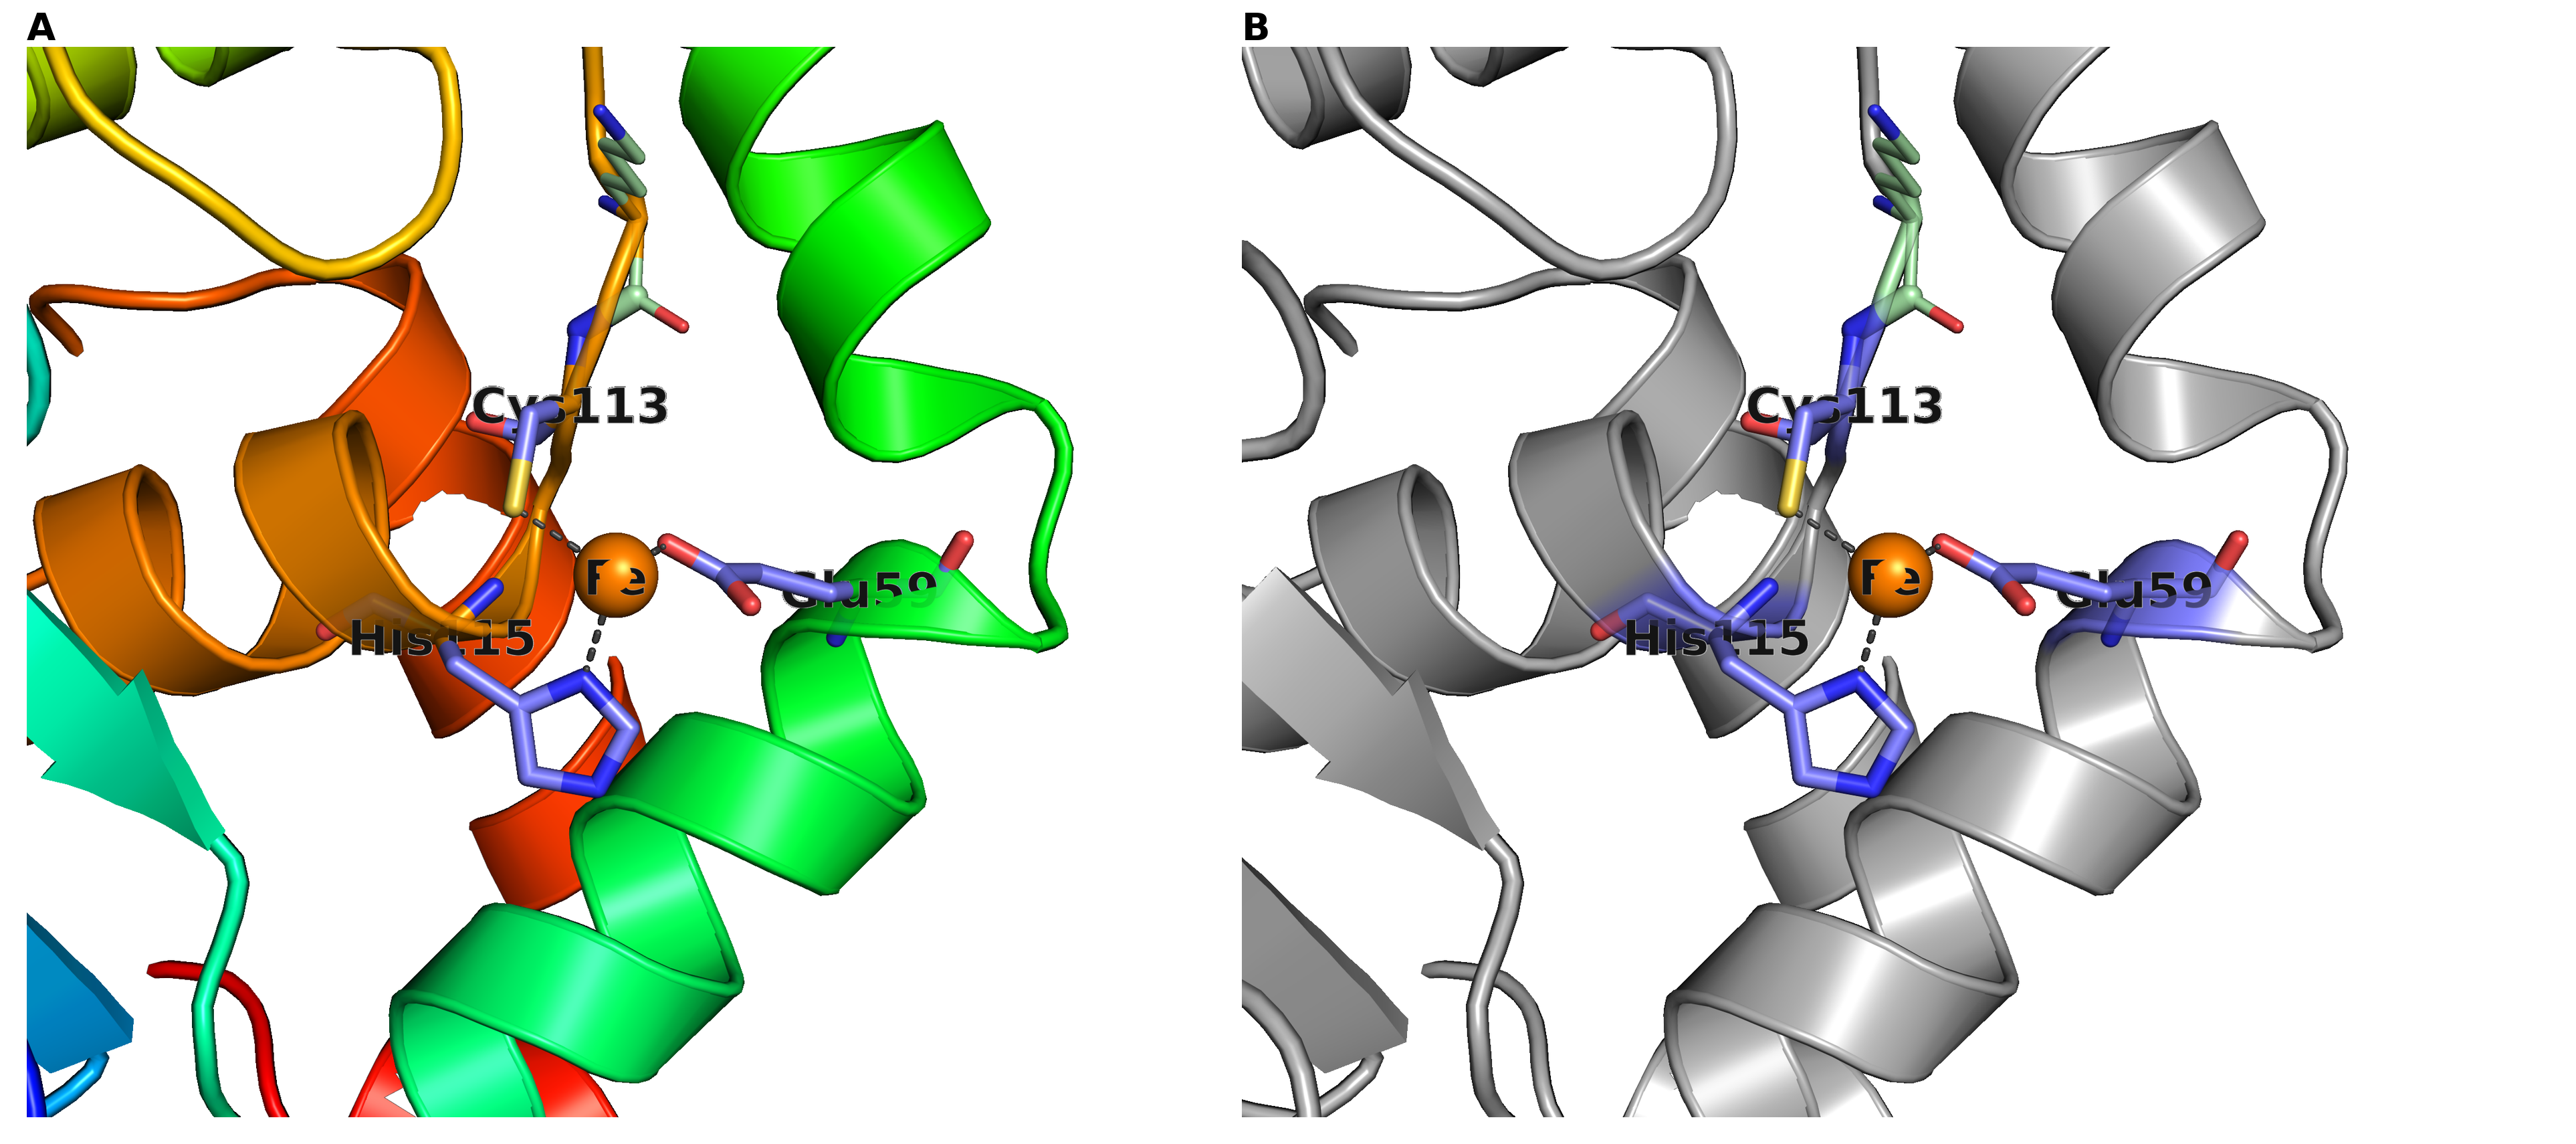
\includegraphics[width=\textwidth]{figures/figure1_active_site.png}
\caption{Le site métallique prédit de Rv1025 (DUF501). \textbf{(A)} Repli AlphaFold global (arc-en-ciel, N vers C) avec les trois résidus coordinateurs du métal représentés en bâtonnets~; la famille n'a aucune structure résolue expérimentalement. \textbf{(B)} Vue rapprochée du modèle holo AlphaFold3 avec le fer~: le métal (sphère orange) est coordonné par les résidus quasi invariants Cys113, His115 et Glu59 (liaisons en pointillés), avec des positions ouvertes faisant face à la poche de seconde sphère conservée. Rendu avec PyMOL}
\label{fig:site}
\end{figure}

\FloatBarrier
\subsection{Le site métallique est une signature universelle de DUF501 bactérien}

Les preuves ci-dessus établissent un site métallique dans une protéine. Que ce site définisse la famille, ou soit une spécialisation mycobactérienne en son sein, est une question différente, qui détermine jusqu'où l'hypothèse fonctionnelle peut être portée. Nous avons donc examiné l'alignement Pfam complet de PF04417 (2~228 segments alignés issus de 2~204 protéines, 471 colonnes, soit environ la moitié des membres InterPro de la famille), dans lequel Rv1025 est présente sous P96375/16--137, de sorte que les trois positions puissent être localisées par ancrage direct plutôt que par réalignement.

La triade est strictement universelle chez les bactéries. Chacune des 1~472 séquences bactériennes quasi complètes porte Glu, Cys et His aux trois positions (100,0~\%), et l'alignement dans son ensemble ne contient aucune substitution non conservative à aucune d'elles~: pas un seul Glu-vers-Asp, et aucun remplacement de Cys113 ni de His115 (Ressource en ligne~9). Les 86 exceptions apparentes sont des gaps plutôt que des substitutions, et 75 d'entre elles tombent dans des fragments de séquence (longueur alignée médiane de 76 résidus contre 124 pour le reste, $p=1\times10^{-46}$). Le site métallique est donc présent dans toute la famille bactérienne, ce qui permet d'énoncer pour DUF501 dans son ensemble une hypothèse fonctionnelle dérivée de Rv1025.

La famille s'étend aussi au-delà des bactéries. Elle inclut 102 membres eucaryotes quasi complets, essentiellement des protistes, parmi eux des parasites apicomplexes (\textit{Babesia}, \textit{Neospora}, \textit{Eimeria}), des straménopiles et \textit{Naegleria}, chez lesquels le domaine est fréquemment enchâssé au sein d'une protéine plus grande. Ce sont des homologues authentiques plutôt que des correspondances de profil marginales, à une identité moyenne de 30~\% à Rv1025 sur le domaine. Trois d'entre eux ont perdu une partie du site, dans les trois cas la paire Cys--His avec rétention du glutamate ($p=2,7\times10^{-4}$ contre les bactéries). Atteindre ce chiffre suppose de coter le site par protéine et non par segment aligné, et cette distinction change le décompte~: 24 accessions de l'alignement y figurent par deux segments couvrant des colonnes complémentaires du profil, le premier portant Glu59 et le second la paire Cys--His, si bien que lire les segments enregistre une perte chez des protéines qui portent les trois résidus. Huit autres segments eucaryotes sont de ce type, et douze segments bactériens aussi, ce qui place le motif dans les deux domaines du vivant et le désigne comme une propriété de la segmentation du profil plutôt que comme un trait eucaryote. Les trois pertes restantes ont été confirmées sur les séquences UniProt entières réalignées au profil, procédure qui a retrouvé la triade complète chez dix accessions de contrôle sur dix (Méthodes). Avec trois cas, nous ne testons pas si la perte suit la divergence de séquence. Les trois sont \textit{Cyclospora cayetanensis}, \textit{Eimeria acervulina} et \textit{Cystoisospora suis}, toutes du sous-ordre apicomplexe Eimeriorina, dont les autres membres de l'alignement (\textit{Besnoitia besnoiti}, \textit{Babesia ovis}, \textit{Neospora caninum}) retiennent le site complet~; aucune des 96 autres protéines eucaryotes quasi complètes ne l'a perdu ($p=1,2\times10^{-4}$, apicomplexes contre autres eucaryotes). La perte est donc rare et taxonomiquement circonscrite, et elle n'est pas ancestrale au sous-ordre. Nous rapportons cette branche eucaryote comme une observation de séquence (Ressource en ligne~10) et ne l'interprétons pas davantage ici~: que ces protéines lient un métal par d'autres moyens, ou pas du tout, n'est pas testé, et la proportion affectée est un majorant car 585 segments alignés n'ont pu se voir assigner de lignée (576 portent la triade complète~; les neuf autres sont des fragments de 37 à 99 résidus alignés, sous le seuil de quasi-complétude, dont deux portent un nom d'entrée d'apicomplexe).

\FloatBarrier
\section{Discussion}

En rassemblant ces résultats, nous proposons que DUF501 est une protéine liant un métal et une métalloenzyme candidate. Les preuves convergent~: un repli sans parent structural (excluant une annotation par homologie), un gène strictement conservé et essentiel à travers les genres d'Actinobactéries, et une constellation quasi invariante Cys--His--Glu dont la géométrie apo et le comportement holo indiquent tous deux un centre métallique divalent, plausiblement catalytique. La catalyse est une hypothèse parmi d'autres (stockage, transfert ou détection du métal, ou rôle structural ou redox), à distinguer expérimentalement. La présence d'un ligand thiol de cystéine est informative~: une coordination par thiolate pointe vers un site à métal de transition, possiblement redox-actif, et est cohérente avec les signaux structuraux faibles et non significatifs précédemment observés pour Rv1025 vis-à-vis des protéines manipulant le métal et le fer. À notre connaissance, c'est la première hypothèse fonctionnelle proposée pour la famille DUF501, et elle illustre une voie générale pour éclairer une famille protéique sombre à travers un seul membre tractable et bien replié lorsque l'homologie structurale échoue~: la conservation à l'échelle des populations projetée sur un modèle à haute confiance, arbitrée par la modélisation holo.

Plusieurs questions restent ouvertes. AlphaFold3 accommode les trois métaux et n'identifie pas, à lui seul, le métal physiologique, bien que le fer produise le modèle le plus confiant et que le ligand thiolate soit compatible avec le fer. La réaction précise catalysée n'est pas établie~; l'architecture de la poche, avec une seconde sphère chargée conservée (Lys112, Arg92), est compatible avec une activité hydrolytique ou redox agissant sur un petit substrat chargé, mais ceci exige un test biochimique. L'association conservée en opéron avec une enzyme glycolytique, une protéine de division et une exopolyphosphatase ne pointe pas vers une voie partagée~: les partenaires prédits les plus forts de chaque protéine se trouvent dans son propre processus (énolase avec la pyruvate kinase, DivIC avec la protéine du divisome FtsQ), aucun régulon de facteur de transcription n'est partagé entre les quatre gènes dans le réseau régulateur de \mtb{}, et la seule association au sein du bloc, Rv1025 avec Ppx2, est portée par des canaux de contexte génomique (voisinage et fusion de gènes) plutôt que par une preuve expérimentale. Le bloc est ainsi co-transcrit mais fonctionnellement hétérogène, et la conservation de son arrangement est compatible avec une sélection au niveau de l'opéron plutôt qu'une fonction biochimique partagée~; notre prédiction négative de complexe argumente spécifiquement contre un hétérodimère stable Rv1025--DivIC, sans exclure une interaction transitoire ou dépendante du contexte du divisome. Un criblage Boltz-2 plus large contre cinq composants supplémentaires du divisome (FtsZ, FtsW, PbpB/FtsI, FtsK, SepF) fut uniformément négatif une fois jugé sur le PAE inter-chaînes plutôt que sur le seul ipTM brut~: le plus haut ipTM nominal du panel (FtsW, 0,281) dépassait le témoin positif interne au panel (DivIC--FtsQ, 0,221), pourtant son PAE inter-chaînes (18,4~\ang{}) était proche du double de celui du témoin (10,4~\ang{}), exactement le piège de l'ipTM sans PAE que le protocole de calibration était conçu pour repérer. Rv1025 ne montre donc aucune preuve de complexe binaire stable avec aucun des composants du divisome testés. Séparément, un test AlphaFold3 direct d'un homodimère de Rv1025, avec et sans les deux ions métalliques holo, n'a de même donné aucune interface confiante (ipTM 0,16, au niveau des témoins de spécificité du monomère), convergeant avec l'analyse de co-évolution ci-dessus sur l'absence d'une interface oligomérique obligatoire capable de compléter la sphère de coordination du métal en trans~; l'état oligomérique reste donc une question ouverte, expérimentalement tractable, plutôt qu'une inférence structurale.

D'un point de vue translationnel, Rv1025 réunit les traits recherchés pour une cible antituberculeuse~: essentialité confirmée à travers les genres, forte vulnérabilité CRISPRi, quasi-invariance à travers les isolats cliniques (limitant la résistance préexistante), un repli ordonné présentant une poche druggable, et une cavité métallique définie et conservée, géométriquement aussi accessible à un ligand exogène que des cibles thérapeutiques dépendantes du zinc établies. Les sites métalliques sont classiquement susceptibles d'inhibition, y compris par des têtes chélatrices du métal, et la voie du polyphosphate à laquelle appartient l'exopolyphosphatase Ppx2 de l'opéron a déjà produit une cible antituberculeuse validée dans la polyphosphate kinase PPK2 \citep{singh2016ppk2target}. DUF501 offre donc un double retour~: une cible thérapeutique candidate chez \mtb{} et le point d'entrée fonctionnel vers toute une famille protéique bactérienne jusqu'alors sombre.

\section{Conclusion}

DUF501 est une famille protéique bactérienne que l'homologie laisse entièrement dans le noir, et dont la trace évolutive se révèle lisible là où l'homologie ne l'est pas. Nous montrons que la famille a un repli nouveau et un arrangement de bloc génique conservé à l'échelle d'un phylum, que son membre chez \mtb{} ne forme pas de complexe binaire stable avec son voisin synténique de division, et qu'il porte un site métallique Cys113--His115--Glu59 non seulement quasi invariant chez ce membre, mais strictement conservé dans chaque séquence bactérienne quasi complète de la famille, sur lequel convergent la modélisation holo et un prédicteur géométrique indépendant de toute information évolutive. Nous proposons que DUF501 est une protéine liant un métal, plausiblement une métalloenzyme~; chez \mtb{}, où le gène est essentiel, vulnérable et quasi invariant à travers les isolats cliniques, ce site est aussi une cible antituberculeuse candidate. Ces conclusions sont computationnelles~; la détermination expérimentale du métal lié, de la structure et de la réaction catalysée est l'étape suivante naturelle, et caractériserait, d'un même geste, une famille protéique conservée à travers les Actinobactéries.

\section*{Déclarations}

\subsection*{Financement}

Cette recherche n'a reçu aucune subvention spécifique d'organismes de financement des secteurs public, commercial ou à but non lucratif.

\subsection*{Intérêts concurrents}

L'auteur déclare n'avoir aucun intérêt concurrent.

\subsection*{Approbation éthique}

Sans objet. Cette étude n'a impliqué ni participants humains, ni données ou tissus humains, ni animaux.

\subsection*{Consentement à participer}

Sans objet.

\subsection*{Consentement à la publication}

Sans objet.

\subsection*{Disponibilité des données et du matériel}

Toutes les données analysées dans cette étude sont publiquement disponibles et sont citées à chaque usage tout au long du Matériel et méthodes, avec les numéros d'accession et les sources de bases de données indiqués sur place. Les sources principales sont l'annotation de référence H37Rv (NC\_000962.3), le modèle AlphaFold de Rv1025 (AlphaFold Protein Structure Database, AF-P96375-F1), la famille InterPro/Pfam PF04417 et son alignement complet, UniProt, et les cribles publiés d'essentialité par transposon et CRISPRi cités dans le texte.

\subsection*{Disponibilité du code}

Les scripts d'analyse (synténie, conservation, génération et analyse des tâches AlphaFold et Boltz-2, rendu des figures) et les résultats intermédiaires tabulaires qui portent les chiffres du texte se trouvent dans le répertoire \texttt{code/} de \url{https://github.com/cguyeux/rv1025-duf501-mtbc}~; un instantané de l'ensemble du projet, sorties de modèles comprises, est archivé sur Zenodo (doi:10.5281/zenodo.22025970).

\subsection*{Contributions des auteurs}

Christophe Guyeux~: conceptualisation, curation des données, analyse formelle, investigation, méthodologie, administration du projet, ressources, logiciel, validation, visualisation, rédaction du brouillon initial, rédaction~: relecture et édition.

\subsection*{Utilisation de l'IA générative et des technologies assistées par IA dans le processus de rédaction}

Lors de la préparation de ce travail, l'auteur a utilisé Claude Code (Anthropic), un environnement logiciel à agent IA reposant sur le modèle Claude Sonnet~5, pour la récupération de données \emph{in silico}, l'analyse statistique, la vérification bibliographique et l'assistance à la rédaction, comme décrit dans la section Matériel et méthodes. Après avoir utilisé cet outil, l'auteur a relu, vérifié de façon indépendante contre les sources primaires et corrigé le contenu autant que nécessaire, et assume l'entière responsabilité du contenu de cette publication.

\bibliographystyle{sn-basic}
\bibliography{references}

\end{document}
